% diag_envelope: TikZ twin of paper/figures/diag_envelope.pdf (generated by diag_common.py).
% Coordinates are inches (y up). Needs \usepackage{tikz}. Body font 7 pt.
\definecolor{dgA}{HTML}{F0F0F0}\definecolor{dgB}{HTML}{DCDCDC}\definecolor{dgC}{HTML}{C4C4C4}
\definecolor{dgAtk}{HTML}{F2C9B8}\definecolor{dgHw}{HTML}{E3EEF7}
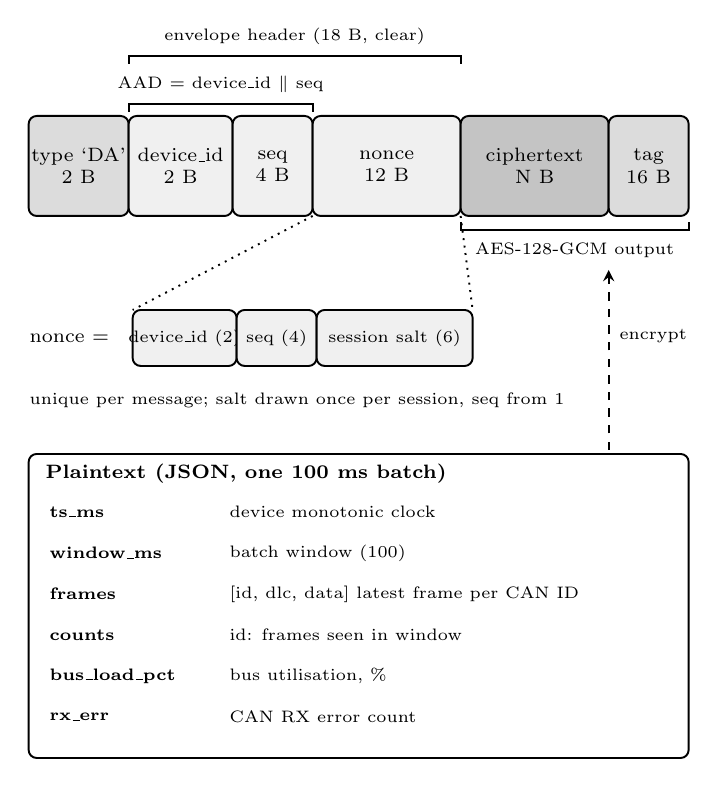
\begin{tikzpicture}[x=1in,y=1in,>=stealth,font=\fontsize{7}{8}\selectfont,line width=0.7pt]
\draw[rounded corners=2.9pt,fill=dgB,line width=0.7pt] (0.100,2.750) rectangle (0.600,3.250);
\node[align=center,inner sep=0pt] at (0.350,3.000) {\fontsize{6.8}{7.6}\selectfont type ‘DA’\\ 2 B};
\draw[rounded corners=2.9pt,fill=dgA,line width=0.7pt] (0.600,2.750) rectangle (1.120,3.250);
\node[align=center,inner sep=0pt] at (0.860,3.000) {\fontsize{6.8}{7.6}\selectfont device\_id\\ 2 B};
\draw[rounded corners=2.9pt,fill=dgA,line width=0.7pt] (1.120,2.750) rectangle (1.520,3.250);
\node[align=center,inner sep=0pt] at (1.320,3.000) {\fontsize{6.8}{7.6}\selectfont seq\\ 4 B};
\draw[rounded corners=2.9pt,fill=dgA,line width=0.7pt] (1.520,2.750) rectangle (2.260,3.250);
\node[align=center,inner sep=0pt] at (1.890,3.000) {\fontsize{6.8}{7.6}\selectfont nonce\\ 12 B};
\draw[rounded corners=2.9pt,fill=dgC,line width=0.7pt] (2.260,2.750) rectangle (3.000,3.250);
\node[align=center,inner sep=0pt] at (2.630,3.000) {\fontsize{6.8}{7.6}\selectfont ciphertext\\ N B};
\draw[rounded corners=2.9pt,fill=dgB,line width=0.7pt] (3.000,2.750) rectangle (3.400,3.250);
\node[align=center,inner sep=0pt] at (3.200,3.000) {\fontsize{6.8}{7.6}\selectfont tag\\ 16 B};
\draw[line width=0.7pt] (0.600,3.270) -- (0.600,3.310) -- (1.520,3.310) -- (1.520,3.270);
\node[align=center,inner sep=0pt] at (1.060,3.410) {\fontsize{6.5}{7.3}\selectfont AAD = device\_id $\Vert$ seq};
\draw[line width=0.7pt] (0.600,3.510) -- (0.600,3.550) -- (2.260,3.550) -- (2.260,3.510);
\node[align=center,inner sep=0pt] at (1.430,3.650) {\fontsize{6.5}{7.3}\selectfont envelope header (18 B, clear)};
\draw[line width=0.7pt] (2.260,2.720) -- (2.260,2.680) -- (3.400,2.680) -- (3.400,2.720);
\node[align=center,inner sep=0pt] at (2.830,2.580) {\fontsize{6.5}{7.3}\selectfont AES-128-GCM output};
\draw[line width=0.7pt,dotted] (1.520,2.750) -- (0.620,2.280);
\draw[line width=0.7pt,dotted] (2.260,2.750) -- (2.320,2.280);
\node[anchor=west,align=flush left,inner sep=0pt] at (0.100,2.140) {\fontsize{6.8}{7.6}\selectfont nonce =};
\draw[rounded corners=2.9pt,fill=dgA,line width=0.7pt] (0.620,2.000) rectangle (1.140,2.280);
\node[align=center,inner sep=0pt] at (0.880,2.140) {\fontsize{6.5}{7.3}\selectfont device\_id (2)};
\draw[rounded corners=2.9pt,fill=dgA,line width=0.7pt] (1.140,2.000) rectangle (1.540,2.280);
\node[align=center,inner sep=0pt] at (1.340,2.140) {\fontsize{6.5}{7.3}\selectfont seq (4)};
\draw[rounded corners=2.9pt,fill=dgA,line width=0.7pt] (1.540,2.000) rectangle (2.320,2.280);
\node[align=center,inner sep=0pt] at (1.930,2.140) {\fontsize{6.5}{7.3}\selectfont session salt (6)};
\node[anchor=west,align=flush left,inner sep=0pt] at (0.100,1.830) {\fontsize{6.5}{7.3}\selectfont unique per message; salt drawn once per session, seq from 1};
\draw[->,line width=0.8pt,dashed] (3.000,1.580) -- (3.000,2.480);
\node[anchor=west,align=flush left,inner sep=0pt] at (3.050,2.150) {\fontsize{6.5}{7.3}\selectfont encrypt};
\draw[rounded corners=2.9pt,fill=white,line width=0.7pt] (0.100,0.040) rectangle (3.400,1.560);
\node[anchor=west,align=flush left,inner sep=0pt] at (0.180,1.460) {\bfseries \fontsize{6.8}{7.6}\selectfont Plaintext (JSON, one 100 ms batch)};
\node[anchor=west,align=flush left,inner sep=0pt] at (0.200,1.270) {\bfseries \fontsize{6.5}{7.3}\selectfont ts\_ms};
\node[anchor=west,align=flush left,inner sep=0pt] at (1.100,1.270) {\fontsize{6.5}{7.3}\selectfont device monotonic clock};
\node[anchor=west,align=flush left,inner sep=0pt] at (0.200,1.065) {\bfseries \fontsize{6.5}{7.3}\selectfont window\_ms};
\node[anchor=west,align=flush left,inner sep=0pt] at (1.100,1.065) {\fontsize{6.5}{7.3}\selectfont batch window (100)};
\node[anchor=west,align=flush left,inner sep=0pt] at (0.200,0.860) {\bfseries \fontsize{6.5}{7.3}\selectfont frames};
\node[anchor=west,align=flush left,inner sep=0pt] at (1.100,0.860) {\fontsize{6.5}{7.3}\selectfont [{id, dlc, data}] latest frame per CAN ID};
\node[anchor=west,align=flush left,inner sep=0pt] at (0.200,0.655) {\bfseries \fontsize{6.5}{7.3}\selectfont counts};
\node[anchor=west,align=flush left,inner sep=0pt] at (1.100,0.655) {\fontsize{6.5}{7.3}\selectfont {id: frames seen in window}};
\node[anchor=west,align=flush left,inner sep=0pt] at (0.200,0.450) {\bfseries \fontsize{6.5}{7.3}\selectfont bus\_load\_pct};
\node[anchor=west,align=flush left,inner sep=0pt] at (1.100,0.450) {\fontsize{6.5}{7.3}\selectfont bus utilisation, \%};
\node[anchor=west,align=flush left,inner sep=0pt] at (0.200,0.245) {\bfseries \fontsize{6.5}{7.3}\selectfont rx\_err};
\node[anchor=west,align=flush left,inner sep=0pt] at (1.100,0.245) {\fontsize{6.5}{7.3}\selectfont CAN RX error count};
\end{tikzpicture}
